%generare il pdf con il comando: pdflatex main.tex
\documentclass[a4paper, oneside, openany]{article}
\usepackage{sos}
\newcommand{\Titolo}{Progetto di Tecnologie Web}

\newcommand{\Gruppo}{TecWeb\&Pastorizia}

\newcommand{\Redazione}{
	Manuel Vianello - 1102466 \newline
	Cavallin Giovanni - 1148957\newline
	Stefano Panozzo - 1097068
}

\newcommand{\ACapoRedazione}{
	Manuel Vianello - 1102466 \newline
	Cavallin Giovanni - 1148957\newline
	Stefano Panozzo - 1097068
}

\newcommand{\Referente}{
Cavallin Giovanni - 1148957 \newline
giovanni.cavallin.1@studenti.unipd.it
	}

\newcommand{\Data}{13 Settembre 2018}

\newcommand{\NomeProgetto}{Progetto di Tecnologie Web}

\newcommand{\Mail}{giovanni.cavallin.1@studenti.unipd.it}

	\newcommand{\DescrizioneDoc}{Documento riportante le informazioni relative al progetto di tecnologie web.}
	
	\newcommand{\versione}{1.0.0}



\begin{document}
\copertina{}
%%%%%%%%%%%%%%%%%%%%%%%%%%%%%%%%%%%%%%%%%%%%%%%%%%%%%%%%%%%%%%%%%%%%%%%%%%%%%%%%%%%%%%%%%%%%%%%%%%%%%%%
%SOMMARIO
\newpage
\tableofcontents
\newpage
%%%%%%%%%%%%%%%%%%%%%%%%%%%%%%%%%%%%%%%%%%%%%%%%%%%%%%%%%%%%%%%%%%%%%%%%%%%%%%%%%%%%%%%%%%%%%%%%%%%%%%%
%PARAGRAFI
\newpage
\section{Introduzione}
Il sito web sviluppato per il progetto di tecnologie web si occupa di fornire delle informazioni relative ad un'azienda agricola di fantasia. Questa azienda produce grano biologico, che si occupa di vendere come business to business, e fornisce alcune attrezzature come terzista per il lavoro nei campi.
Lo scopo principale di questo sito è quello di intercettare un bacino d'utenza che in genere fatica a reperire le informazioni qui presentate, perché trasmesse principalmente come passaparola nell'ambiente contadino. Inoltre si occupa di dare visibilità all'azienda agricola, che altrimenti non avrebbe modo di presentarsi in veste web.
~\\ ~\\
Per accedere al sito recarsi all'indirizzo:\\ \url{https://tecweb2016.studenti.math.unipd.it/mvianell/}.~\\ ~\\
Per poter accedere al pannello di amministrazione, del quale link è a fondo pagina, si devono usare le seguenti credenziali:\\ 
\textbf{username}: admin@admin.com\\ 
\textbf{password}: admin
\section{Processi primari}
\subsection{Processo di fornitura}

\subsubsection{Studio di Fattibilità}
Si tratta del documento in cui vengono analizzati tutti i capitolati, valutandone pregi e difetti, allo scopo di scegliere quello di maggiore affinità per il gruppo.
Dopo che il \RdP{} (il cui ruolo è descritto nel paragrafo \ref{responsabile_progetto}) avrà riunito il team e discusso con esso di tutti i capitolati, gli \anas{} avranno il compito di stilare lo \SdF{} seguendo le considerazioni emerse.\\
Lo \SdF{} sarà organizzato come segue:
\begin{itemize}
	\item \textbf{Informazioni sul capitolato}:
	Vengono ricordati il nome del \emph{progetto}\ped{G}, il \textit{proponente}\ped{G} e i \textit{committenti}\ped{G};
	\item \textbf{Descrizione}:
	Si riassume lo scopo del capitolato;
	\item \textbf{Dominio applicativo}:
	Si specifica il settore di utilizzo del prodotto finale;
	\item \textbf{Dominio tecnologico}:
	Si elencano le tecnologie che dovranno essere utilizzate nello sviluppo del capitolato;
	\item \textbf{Aspetti positivi}:
	Si elencano i motivi che il gruppo potrebbe considerare vantaggiosi;
	\item \textbf{Aspetti negativi}:
	Si elencano le potenziali criticità che il gruppo dovrà tenere in considerazione nella scelta finale;
	\item \textbf{Valutazione finale}:
	Si analizzano gli aspetti positivi e quelli negativi riscontrati e si motiva l'eventuale approvazione o esclusione.
\end{itemize}

\subsubsection{Rapporti con il proponente}
Una volta scelto il capitolato, si intende instaurare un rapporto quanto più costante e profittevole con la \proponente{} allo scopo di:
\begin{itemize}
	\item Stabilire un accordo in merito allo sviluppo, al mantenimento, al funzionamento e alla consegna del prodotto;
	\item Realizzare un prodotto che soddisfi totalmente i requisiti obbligatori concordati e quanto più possibile quelli desiderabili;
	\item Stimare i costi;
	\item Concordare la qualifica del prodotto.
\end{itemize}

\subsubsection{Collaudo e consegna del prodotto}
Una volta terminate le fasi di sviluppo, verifica e validazione si effettuerà il collaudo al fine di dimostrare che tutti i requisiti obbligatori e, possibilmente, anche alcuni dei requisiti opzionali siano stati soddisfatti. 
\\In questa fase inoltre si dovrà dimostrare che l'esecuzione di tutti i test di validazione abbia dato un'esito positivo.
\\Il team consegnerà in ultima il prodotto finale su un supporto fisico ai committenti \committenti.

\subsection{Processo di sviluppo}
\subsubsection{Attività}
\paragraph{Analisi dei Requisiti}
	~\\Gli \anas, una volta terminato lo \SdF, dovranno stilare l'\AdR, che si dovrà attenere alle seguenti regole: \\
	~\\ \textbf{Classificazione dei Requisiti}:
	i requisiti saranno classificati secondo la seguente codifica:
		\begin{center}
			R[Importanza][Tipo][Codice]
		\end{center}
	dove:
	\begin{itemize}
		\item \textbf{Importanza} può assumere questi valori:
			\begin{itemize}
				\item F: indica un requisito funzionale;
				\item Q: indica un requisito di qualità;
				\item P: indica un requisito prestazionale;
				\item V: indica un requisito di vincolo.
			\end{itemize}
		\item \textbf{Tipo} può assumere questi valori:
			\begin{itemize}
				\item O: indica un requisito obbligatorio;
				\item D: indica un requisito desiderabile;
				\item F: indica un requisito facoltativo.
			\end{itemize}
		\item \textbf{Codice} indica il codice identificativo del requisito, è univoco e deve essere indicato in
		forma gerarchica.
	\end{itemize}
	Per ogni requisito si dovrà inoltre indicare una breve descrizione e la fonte, che può essere una tra le seguenti:
		\begin{itemize}
		\item Capitolato: deriva direttamente dal testo del capitolato;
		\item Verbale: deriva da un incontro verbalizzato;
		\item Interno: deriva da discussioni interne al team.
		\end{itemize}
	
	~\\ \textbf{Classificazione dei casi d'uso}: i casi d’uso saranno classificati secondo la seguente codifica:
		\begin{center}
			UC[Codice padre].[Codice identificativo]
		\end{center}
	dove:
		\begin{itemize}
			\item Codice padre: indica il codice del caso d’uso padre di quello in esame, se non è identificabile è da omettere;
			\item Codice identificativo: codice univoco e progressivo del caso d’uso in esame.
		\end{itemize}
	Per ogni caso d’uso saranno inoltre identificate le seguenti informazioni:
		\begin{itemize}
			\item \textbf{Attori}: indica gli attori coinvolti nel caso d’uso;
			\item \textbf{Descrizione}: chiara, precisa e concisa descrizione del caso d’uso;
			\item \textbf{Precondizione}: indica la situazione che deve essere vera prima dell’esecuzione del caso d’uso;
			\item \textbf{Flusso principale degli eventi}: descrizione composta dal flusso dei casi d’uso figli;
			\item \textbf{Postcondizione}: indica la situazione che deve essere vera dopo l’esecuzione del caso d’uso;
			\item \textbf{Estensioni}: indica quali sono tutte le estensioni, se presenti;
			\item \textbf{Generalizzazioni}: indica quali sono tutte le generalizzazioni, se presenti.
		\end{itemize}
	
\paragraph{Progettazione}
	~\\I \progs{} (il cui ruolo è descritto nel paragrafo \ref{progettista}) dovranno delinerare i requisiti utili alla documentazione specifica e determinare le linee guida da seguire.
	~\\La progettazione ha come scopo quello di soddisfare le peculiarità identificate durante l'\AdR. Un altro obiettivo è quello di realizzare un prodotto \emph{manutenibile}\ped{G} ovvero, un 
	 che abbia una struttura in grado di facilitare i cambiamenti futuri.
	\\Infine deve realizzare al meglio i requisiti di qualità imposti dal committente.
	\subparagraph{Linee guida per la progettazione}
	Dopo aver completato l'\AdR{} i \progs{} dovranno sottostare alle seguenti linee guida per lo sviluppo dell'architettura logica del sistema:
	\begin{itemize}
		\item Si dovrà puntare ad una progettazione chiara e di immediata comprensione;
		\item Le componenti progettate dovranno essere quanto più riutilizzabili e manutenibili;
		\item La complessità non dovrà mai essere intrattabile;
		\item I \progs{} dovranno rientrare nei costi e nelle risorse disponibili;
		\item I \progs{} dovranno descrivere i \emph{design pattern}\ped{G} che intendono utilizzare per la realizzazione dell'architettura, fornendone una breve descrizione e un diagramma.
	\end{itemize}
\begin{comment}
	\subparagraph{UML}
	~\\Le tipologie di diagrammi \emph{UML}\ped{G} che verranno adoperate per analizzare, descrivere e specificare le scelte progettuali adottate saranno:
	\begin{itemize}
		\item \textbf{Diagrammi di classe}:
		\item \textbf{Diagrammi di } \emph{\textbf{package}}\ped{G}: documentano le dipendenze tra le classi ed è utile per controllare la complessità strutturale in sistemi medio-grandi;
		\item \textbf{Diagrammi di attività}: modellano un processo e organizzano più entità in un sistema di azioni secondo un determinato flusso. I diagrammi delle attività sono un tipo particolare di \emph{diagramma di stato}\ped{G} che identifica la variazione di stato al verificarsi di alcune condizioni legate ad una o più entità;
		\item \textbf{Diagrammi di sequenza}: descrivono la collaborazione di un gruppo di oggetti che devono implementare collettivamente un comportamento. Sono diagrammi molto semplici, ma che permettono di capire se l'architettura creata viene eseguita.
	\end{itemize}

	\paragraph{Codifica}
	~\\In questa fase i \progrs{} (il cui ruolo è descritto nel paragrafo \ref{programmatore}), seguendo le norme delineate nella progettazione, devono realizzare il passaggio dalla fase di pianificazione all'effettiva realizzazione del prodotto.
	Le norme qui presenti serviranno come strumento per realizzare un codice uniforme e di alta qualità. Inoltre, per mantenerne la manutenibilità, dovrà essere realizzato in inglese.
	I \progrs{} si dovranno attenere agli standard di codifica qui di seguito elencati.
	\subparagraph{Nomi}
	\begin{itemize}
		\item Ogni elemento deve avere un nome rappresentativo e pertinente alla funzione da esso svolta;
		\item Si dovrà utilizzare la notazione \emph{CamelCase}, ovvero la concatenazione di più parole, ognuna delle quali con lettera iniziale maiuscola. In caso di metodi e variabili la prima lettera dovrà essere minuscola, mentre per le classi maiuscola;
		\item Si potranno utilizzare singole lettere esclusivamente per identificare gli indici dei cicli;
		\item Saranno da evitare notazioni troppo simili tra di loro in significato e denominazione;
		\item Si dovranno evitare errori di ortografia.
	\end{itemize}
	\subparagraph{Commenti}
	~\\Sarà necessario che il codice contenga dei commenti esplicativi per facilitarne la comprensione.
	\newline In particolare, si dovranno seguire queste linee guida:
	
	\begin{comment}
	\begin{itemize}
		\item \textcolor{red}{lista di linee guida per i commenti}
	\end{itemize}
	\end{comment}
	
	\subparagraph{Formattazione}
	\begin{itemize} 
		\item Il rientro predefinito dovrà essere di un \emph{Tab} per allineare le sezioni di codice;
		\item La parentesi graffa di apertura sarà alla fine della riga, mentre quella di chiusura a capo;
		\item Prima e dopo ogni operatore dovrà esserci uno spazio);
		\item I blocchi saranno tra loro spaziati per una maggiore comprensione;
%		\item Il codice sorgente dovrà essere quanto più suddiviso in file e dovrà essere raggruppato in sottocartelle che dovranno rispecchiare il pattern utilizzato.
%		\item \textcolor{red}{Se ce ne sono altre le inseriamo qui. Da pensare al pattern, }
	\end{itemize}
\subsubsection{Strumenti}
Gli strumenti utilizzati durante la fase dei processi primari sono:
\begin{itemize}
	\item \textbf{TexStudio}
	\newline Il gruppo ha scelto \emph{TexStudio} come editor multipiattaforma per comporre i documenti in \emph{\LaTeX}\ped{G};
	\item \emph{\textbf{\emph{SWEgo}}}\ped{G} \footnote{\href{https://www.swego.it/}{https://www.swego.it/}}
	~\\ Il gruppo ha scelto \emph{SWEgo} come database per la gestione dei casi d'uso, dei requisiti e del loro tracciamento per il documento \AdR{}. Dopo un'attenta analisi preliminare dello strumento il team ha deciso di utilizzarlo nonostante alcuni problemi rilevati nella generazione del codice \LaTeX{} perché, permette una stesura standardizzata e sempre aggiornata di alcuni capitoli importanti del documento, a fronte di correzioni minori e applicabili in maniera seriale e regolamentata;
	\item \textbf{Astah}\ped{G}
	~\\Il gruppo ha scelto l'utilizzo di \emph{Astah} per la generazione dei diagrammi dei casi d'uso dell'\AdR{};
	\item \textbf{Microsoft Excel 365}
	\newline Il gruppo ha scelto di utilizzare \emph{Microsoft Excel 365}\ped{G} per la generazione di grafici e di tabelle da poter inserire all'interno del \PdQ{} e \PdP{} perché di immediata realizzazione e visualizzazione;
	\item \textbf{Instagantt} \footnote{\href{https://instagantt.com/}{https://instagantt.com/}}
	~\\Instagantt è un servizio web fortemente legato ad Asana (vedi descrizione negli strumenti dei \emph{processi organizzativi}), strumento con il quale si integra perfettamente, nonostante sia disponibile anche una versione \emph{standalone}\ped{G}. Esso permette di creare diagrammi di Gantt e gestire in maniera semplificata la timeline e la struttura di un progetto.
	\item \textbf{Visual Studio Code} \footnote{\href{https://code.visualstudio.com/}{https://code.visualstudio.com/}} 
	~\\Visual Studio Code è un editor di testo gratuito e multipiattaforma che supporta operazioni di debugging e di versionamento. Permette inoltre di installare vari pacchetti che consentono di personalizzarne l'usabilità e di supportare nuove tecnologie o linguaggi di programmazione. Il gruppo lo ha scelto come editor di testo per scrivere il codice in React e Redux.
	\item \textbf{Truffle} \footnote{\href{http://truffleframework.com/}{http://truffleframework.com/}}
	~\\Truffle è un ambiente di sviluppo e testing per Ethereum. Il gruppo ha deciso di utilizzarlo perché fornisce un aiuto nello sviluppare, pubblicare e testare gli smart contract.
	\item \textbf{Ganache} \footnote{\href{http://truffleframework.com/ganache/}{http://truffleframework.com/ganache/}}
	~\\Ganache è uno strumento legato a Truffle che consente di avere una blockchain virtuale locale utilizzabile per sviluppare contratti, applicazioni ed effettuare dei test. Permette anche di generare degli account di testing  utilizzabili  durante lo sviluppo.
	\item \textbf{Npm} \footnote{\href{https://www.npmjs.com/}{https://www.npmjs.com/}}
	~\\npm è un gestore di pacchetti per il linguaggio Javascript.
	
	\item \textbf{Remix}
	~\\Remix è l'ambiente di sviluppo integrato ufficiale di Ethereum per il linguaggio di programmazione di smart contract \textit{solidity}\ped{G}. Viene eseguito all'interno di un browser web, online all'indirizzo  \url{https://remix.ethereum.org/} oppure in locale scaricando i relativi file sulla propria macchina.% Il gruppo ha deciso di utilizzarlo in locale perché c'è il vantaggio di poter comunicare con un nodo client di ethereum eseguito in locale.
\end{itemize}	


\newpage
\section{Progettazione}
\subsection{Studio dell'utenza finale}
\subsubsection{Utente generico}
L'utenza maggiore che ci si aspetta potrà visitare questo sito è composta principalmente da persone dal profilo informatico medio basso alla ricerca di informazioni dettagliate riguardo la fornitura dell'azienda, probabilmente in mobilità. L'applicativo web offre informazioni relative ad un'azienda agricola, posto che in genere non è frequentato pubblicamente per svago. Per questo motivo la maggior parte delle informazioni sono contenute in pagine statiche. Inoltre si sono create le pagine di \textbf{servizi} e \textbf{prodotti} che, pur non permettendo un acquisto o una prenotazione on line, offrono all'utente la possibilità di vedere le offerte e di contattare l'azienda telefonicamente nella scheda \textbf{contattaci}.
\subsubsection{Azienda business-to-business}
Ci si può aspettare inoltre che qualche azienda in cerca di un commercio business-to-business di grano visiti il sito. In questo caso le pagine statiche di \textbf{home} e \textbf{chi siamo} offrono una panoramica sulla storia e sulla solidità dell'azienda, pubblicizzandola. Ci si aspetta quindi un utente più esperto nell'utilizzo di un PC o smartphone, che quindi potrà eventualmente anche creare un messaggio con più informazioni, in attesa di un contatto telematico, sfruttando il form preparato nella scheda \textbf{contattaci}.
\subsubsection{Amministratore}
Il sito potrà essere gestito da uno o più amministratori ingaggiati dall'azienda, che si supporranno essere persone mediamente più esperte nell'utilizzo di un computer, che si occuperanno di amministrare il sito da una postazione principalmente fissa anche se, tuttavia, la parte amministrativa del sito è navigabile anche attraverso tablet e smartphone.

\subsection{Layout del sito}
Sebbene abbastanza simili sotto il punto di vista del layout, la struttura presentata agli utenti generici e agli amministratori varia di un po'. Prenderemo in esame i due layout in maniera distinta.
\subsubsection{Utente generico}
\paragraph{Barra di navigazione}
~\\Il sito è stato pensato per avere una navigazione a barra orizzontale fissa posta in alto sullo schermo. Le pagine del sito sono, per quanto riguarda gli utenti non registrati:
\begin{itemize}
	\item \textbf{Home}
	\item \textbf{Chi siamo}
	\item \textbf{Prodotti}
	\item \textbf{Servizi}
	\item \textbf{Contattaci}
\end{itemize}
Nella barra è presente il logo dell'azienda e i pulsanti che portano alle altre pagine del sito. In particolare, il pulsante indicante la pagina attuale è incorniciato, mentre gli altri, se il mouse ci passa sopra, vengono sottolineati. All'interno della barra, posto subito sotto, è presente il breadcrumb: a sinistra si occupa di indicare la posizione attuale all'interno del sito, a destra è presente un'ancora che porta direttamente al contenuto. Se si utilizza il \emph{tab} da tastiera si potrà apprezzare che questo è il primo link cliccabile. Nell'immagine seguente è possibile vedere un esempio della barra:
\begin{figure}[h!]
	\centerline{
\includegraphics[scale=0.45]{img/barra_navigazione.jpg}}
	\caption{Barra di navigazione per l'utente generico}
	\label{fig:navbarGU}
\end{figure}
~\\Sebbene non facente parte della barra, è presente un'àncora fissata in basso a destra sul sito che si occupa di riportare il lettore all'inizio del contenuto.
\begin{figure}[h!]
	\centerline{
\includegraphics[scale=0.45]{img/jump_to_menu.jpg}}
	\caption{Ancora all'inizio del contenuto}
	\label{fig:anchor}
\end{figure}
\paragraph{Corpo}
~\\Il corpo è disposto con layout orizzontale all'interno della pagina, con una larghezza massima fissata, in modo da renderlo più elegante anche con risoluzioni elevate. La maggior parte dei contenuti è organizzata in rettangoli, ognuno dei quali contiene il titolo della sotto sezione, il testo e un'immagine indicativa.
Nell'immagine subito successiva si può notare un esempio:
\begin{figure}[h!]
	\centerline{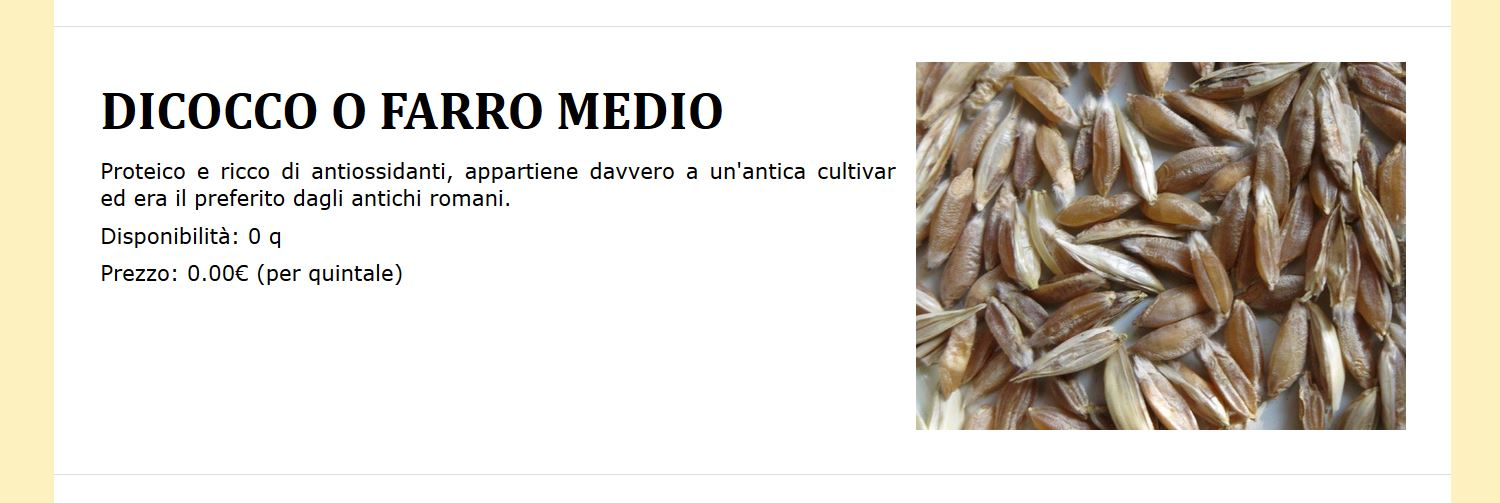
\includegraphics[scale=0.40]{img/corpo_esempio.jpg}}
	\caption{Esempio di sezione del corpo}
	\label{fig:corpoGU}
\end{figure}
\paragraph{Pié di pagina}
~\\A pié di pagina si possono trovare delle informazioni relative al progetto, ovvero il nome dei partecipanti alla creazione del sito e le certificazioni di adesione agli standard \emph{XHTML} e \emph{CSS3}. Inoltre è presente un collegamento alla sezione di amministrazione, alla quale si può accede solo se già registrati da un altro amministratore.
\begin{figure}[h!]
	\centerline{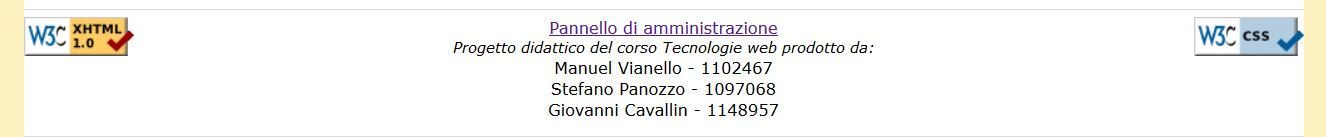
\includegraphics[scale=0.45]{img/footer.jpg}}
	\caption{Pié di pagina del sito}
	\label{fig:footer}
\end{figure}
\subsubsection{Amministratore}
La GUI si differenzia da quella dell'utente base per alcune particolarità.
\paragraph{Barra di navigazione}
~\\Al posto delle pagine sopra illustrate ci sono altre pagine in cui navigare:
\begin{itemize}
	\item \textbf{Pannello amministrazione}
	\item \textbf{Prodotti}
	\item \textbf{Servizi}
	\item \textbf{Storico prenotazioni}
	\item \textbf{Prenotazioni}
	\item \textbf{Clienti}
	\item \textbf{Amministratori}
\end{itemize}
Nel breadcrumb poi, al posto del \emph{Vai al contenuto}, sono presenti due link: un \emph{Torna al sito} e un pulsante di \emph{Logout}, che hanno lo stesso risultato di riportare l'utente al sito generico, ma che nel secondo caso chiude la sessione di amministratore. Viene infine rimossa l'àncora per tornare all'inizio della pagina.
\begin{figure}[h!]
	\centerline{
\includegraphics[scale=0.49]{img/barra_navigazione_admin.jpg}}
	\caption{Barra di navigazione per l'amministratore}
	\label{fig:navbarAD}
\end{figure}
\paragraph{Corpo}
~\\La struttura rimane pressoché invariata, ma in ognuna di esse - meno la \textbf{Storico prenotazioni} - è presente a fondo pagina un modulo di aggiunta informazioni.
\begin{figure}[h!]
	\centerline{
\includegraphics[scale=0.49]{img/add_form.jpg}}
	\caption{Form di aggiunta informazioni}
	\label{fig:addForm}
\end{figure}
\paragraph{Pié di pagina}
~\\Nel pié di pagina invece viene solamente rimosso il link al pannello di amministrazione poiché inutile.

\subsection{Contenuti veicolati}
Dal punto di vista dei contenuti veicolati invece il sito presenta una profonda differenza a seconda del destinatario a cui si riferisce. Prenderemo in esame un utente alla volta.
\subsubsection{Utente generico}
I contenuti destinati all'utente generico possono essere statici o dinamici:
\paragraph{Contenuti statici}
\subparagraph{Home}
~\\È una rapida overview delle informazioni relative all'azienda. Quindi è presente il logo, che la identifica anche visivamente, e un riepilogo di come l'azienda si preoccupa di coltivare i propri prodotti.
\subparagraph{Chi siamo}
~\\È una presentazione un po' più approfondita dell'azienda, dove vengono descritte le origini della stessa e la sua mission, per così dire, ovvero l'agricoltura biologica.
\subparagraph{Contattaci}
~\\È una pagina dei contatti, dove l'utente può mettersi direttamente in contatto con l'azienda attraverso un form da compilare, oppure potendo chiamare il numero di telefono disponibile. Per utilizzare il form è necessario che nel server in cui è hostato il sito sia predisposto un mail server. Come conferma dell'effettivo invio del form, si riceverà una copia della richiesta appena effettuata all'azienda Cavallin. Eventualmente è comunque possibile utilizzare il link sottostante oppure il numero di telefono.
\paragraph{Contenuti dinamici}
\subparagraph{Prodotti} 
~\\Presenta tutti i prodotti di cui l'azienda dispone al momento attuale e dei quali si occupa della coltivazione. Essendo possibile per l'azienda variare coltivazioni, si è pensato di rendere questi contenuti dinamici così da poterli aggiuntere, rimuovere o aggiornare dall'amministrazione. Sono correlati dal nome, una breve descrizione, un'immagine significativa, il prezzo al quintale e dalla disponibilità.
\subparagraph{Servizi} 
~\\Offre una visione delle attrezzature delle quali l'azienda dispone. Essendo disponibile un servizio da terzista, un eventuale cliente può vedere gli attrezzi e poi accordarsi con l'azienda attraverso il form di contatti. Questa parte verrà descritta nella parte di amministrazione.

\subsubsection{Amministrazione}
I contenuti destinati all'amministrazione sono solamente dinamici, poiché fortemente legati allo stato dei prodotti, dei servizi e delle prenotazioni. Un amministrazione ha a disposizione le pagine di:
\paragraph{Pannello amministrazione} viene presentata un riassunto di ciò che è possibile fare accedendo alla parte amministrativa del sito.
\paragraph{Prodotti}
~\\Viene visualizzata la lista dei prodotti attualmente disponibili ma senza immagini, poiché non troppo rilevanti al fine delle modifiche. Per ogni prodotto è possibile impostarne un nuovo prezzo al quintale e una nuova disponibilità. Inoltre è possibile eliminare la cultivar, qualora non ce ne fosse più bisogno, e aggiungerne una nuova, per la quale è necessario inserire tutti i campi disponibili: nome, quantità, prezzo e un'immagine.
\paragraph{Servizi}
~\\Viene visualizzata la lista dei macchinari attualmente presenti in azienda. Come per i prodotti, è possibile modificarne il prezzo all'ora, si possono eliminare e se ne possono inserire di nuovi, compilando tutti i campi del form a fondo pagina.
\paragraph{Amministratori}
~\\È possibile per gli amministratori la gestione degli altri amministratori, che possono quindi essere aggiunti o eliminati in questa pagina.
\paragraph{Clienti}
~\\La parte amministrativa del sito permette la gestione di ordini di macchinari da parte di clienti per una certa quantità di tempo. Per questo motivo è presente una sezione \textbf{Clienti}, che si occupa di aggiungere tutte le informazioni relative ad un cliente che precedentemente si è dimostrato interessato all'azienda, e attraverso il quale poi è possibile effettuare la prenotazione vera e propria, che quindi attesta l'utilizzo di un determinato servizio da parte di un cliente ben preciso.
\paragraph{Prenotazioni}
~\\Qui si possono visualizzare le prenotazioni attualmente attive, oppure se ne può aggiungere una nuova: in questo caso bisogna selezionare il macchinario, sincerarsi della sua disponibilità, selezionare un cliente e le date di inizio e fine della richiesta. Non si possono ovviamente selezionare servizi attualmente attivi.
\paragraph{Storico prenotazioni}
~\\In questa sezione si possono visualizzare le prenotazioni passate: in questa maniera si può avere uno storico, utile per il gestore dell'azienda. Ovviamente quese prenotazioni non influiscono sullo stato dei macchinari, che quindi possono essere selezionabili durante la generazione di una prenotazione.












\section{Processi organizzativi}
\subsection{Processo di coordinamento}

\subsubsection{Comunicazioni}
\paragraph{Comunicazioni interne}
	Per gestire le comunicazini interne si è riscontrata la necessità di distinguere la modalità di presentazione delle informazioni in:
	\begin{itemize}
	\item\textbf{Comunicazione formale}: questa modalità viene usata per le discussioni ufficiali ed inerenti a gestione e sviluppo del progetto; 
	\item\textbf{Comunicazione informale}: questa modalità viene usata per scambiare informazioni non ufficiali e discutere riguardo le attività di progetto.
	\end{itemize}
	
	Si è deciso di utilizzare i seguenti strumenti:
	\begin{itemize}
	\item\textbf{\textit{Telegram}}\ped{G};
	\item\textbf{\textit{Slack}}\ped{G}.
	\end{itemize}
	
\paragraph{Comunicazioni esterne}
\begin{itemize}
\item\textbf{Email}: è stato creato l'indirizzo di posta elettronica:
\textbf{\emailgruppo}

L'utilizzo di tale casella di posta è affidato unicamente al \RdP, per la gestione delle relazioni con il committente ed il  proponente del progetto.

Le email dovranno avere la seguente forma:
	\begin{itemize}
	\item\textbf{Oggetto}: l'oggetto dev'essere chiaro e conciso, per riconoscere e distinguere facilmente tra loro le email;
	\item\textbf{Apertura}: ogni email deve iniziare con un aggettivo di circostanza seguito dal titolo e dal  nome del destinatario,  oppure con un saluto formale e terminare con una virgola;
	\item\textbf{Corpo}: nel corpo, che deve essere breve ed esaustivo, verranno spiegate le ragioni per cui si sta scrivendo l'email;
	\item\textbf{Allegati}: è possibile l'invio di allegati, su richiesta del proponente o del committente;
	\item\textbf{Chiusura}: la chiusura deve essere separata dal corpo con il doppio ritorno a capo e prevede un congedo formale e la firma del mittente.
	\end{itemize}

\item\textbf{Slack}: verrà utilizzato, su richiesta del committente, per lo scambio di informazioni in maniera ufficiosa.
\end{itemize}

\subsubsection{Riunioni}
\paragraph{Obiettivi}
~\\Le riunioni sono di fondamentale importanza per la gestione di un progetto. È indispensabile che i membri del team abbiano
modo di confrontarsi tra loro al fine di risolvere i problemi esistenti e generare nuove idee. Una riunione è inoltre un
ottimo mezzo per creare armonia e consolidare i rapporti all'interno del gruppo. Le riunioni con il proponente/i o committente/i avranno invece lo scopo di condividere gli obiettivi raggiunti e di confrontarsi nel caso in cui si presenti
la necessità di colmare lacune. 
\paragraph{Riunioni interne}
~\\Per un produttivo svolgimento delle riunioni interne, verranno rispettati i seguenti ruoli:
\begin{itemize}
\item\textbf{Moderatore}: il \RdP{} ha il dovere di convocare il team alle riunioni interne quando necessario per un confronto tra i vari membri;
durante gli incontri è richiesto che tutti i membri siano presenti, salvo eccezioni precedentemente segnalate.
Il \RdP{} avrà quindi l'obbligo di seguire l'ordine del giorno riguardo agli argomenti da affrontare 
%\textcolor{red}{da fungere da moderatore QUESTO IL MODERATORE LO FA?}, 
e di trovare un consenso unanime riguardo le decisioni da prendere.
Per svolgere il prorio compito in maniera adeguata, il moderatore è tenuto ad avere un atteggiamento autorevole, flessibile
e diligente;
\item\textbf{Segretario}\ped{G}: il \emph{Segretario} ha il compito di stendere una prima minuta dell'incontro, controllare che venga seguito punto per punto l'ordine del giorno e redigere la versione finale del \emph{verbale}\ped{G}.
Conclusa una riunione, il \emph{Segretario} avrà inoltre il compito di fornire una copia del verbale ad ogni membro del team,
comprendente un resoconto delle decisioni prese e degli obiettivi prefissati;
\item\textbf{Partecipanti}: i partecipanti sono tenuti a presenziare puntualmente qualora venga convocata una riunione da parte del \RdP{}. Nel caso in cui un membro sia impossibilitato a partecipare è invitato
a comunicarlo tempestivamente al \RdP, al fine di accordarsi sul come procedere. È richiesto ai partecipanti di
tenere un comportamento diligente e responsabile per un corretto svolgimento dell'assemblea.
\end{itemize}

\subparagraph{Descrizione}
~\\Le riunioni dovranno avere cadenza settimanale, per fare il punto della situazione riguardo gli obettivi prefissati e
le difficoltà incontrate. Il \RdP{}, dovrà informare i vari membri della riunione tramite email e questi saranno tenuti a rispondere confermando la presenza o motivando l'assenza. Una riunione verrà effettivamente considerata
valida solo nel caso in cui siano presenti almeno la metà dei membri convocati. Nel caso contrario, sarà proposta una seconda data all'interno della settimana per ripetere e validare l'incontro.
Le riunioni dovranno concentrarsi su quattro punti cardine:
\begin{itemize}
	\item Informare i membri riguardo le novità;
	\item Valutare il lavoro precedentemente fatto;
	\item Prendere decisioni collettive riguardo eventuali problematiche;
	\item Progettare il percorso per raggiungere gli obiettivi prefissati entro le tempistiche stabilite.
\end{itemize}
Al termine di ogni riunione verrà quindi redatto il corrispondente verbale ed inviato per mail a tutti i membri del team.

\paragraph{Riunioni esterne}
\subparagraph{Descrizione}
Le riunioni con il proponente hanno la funzione di supportare il gruppo di progetto e di consolidare il rapporto tra entrambe le parti. Durante le riunioni, il gruppo avrà l'impegno di condividere gli obiettivi raggiunti e le eventuali problematiche incontrate. 
Il \RdP{} avrà il dovere di convocare le riunioni quando necessario, anche confrontandosi in base alle esigenze dei membri del team. Il segretario scelto invece avrà il compito di verbalizzare quanto emerso dalla discussione, e le possibili richieste di cambiamento e/o correzione emesse dal proponente.

\subsection{Processo di pianificazione}
\subsubsection{Descrizione}
Lo sviluppo di un progetto prevede la cooperazione di diversi ruoli. Per una comprensione unanime del progetto, ogni membro del team dovrà esercitare obbligatoriamente tutti i ruoli previsti, durante periodi temporali differenti, che saranno di seguito elencati. Nel caso in cui sorga la necessità, un membro potrà ricoprire più di un ruolo contemporaneamente, ma solo nel caso in cui non si tratti di redattore e verificatore. Questo caso in particolare è considerato un controsenso, in quanto la figura del verificatore risulterebbe corrotta nell'analisi dei propri documenti. Inoltre, ogni ruolo avrà incarichi diversi, i quali verranno gestiti ed assegnati dal \RdP{} con l'ausilio di opportuni strumenti, in modo da garantire monitoraggio, controllo e revisione del progetto per tutta la sua durata.
\subsubsection{Ruoli}
\paragraph{Responsabile} \label{responsabile_progetto}
Il \RdP{} è colui che detiene la responsabilità sul lavoro svolto dal team, mantiene i contatti esterni e presenta al committente il progetto finale. Egli possiede il potere decisionale e si fa carico dei seguenti oneri:
\begin{itemize}
	\item Pianificazione, coordinamento e controllo delle attività;
	\item Gestione e controllo delle risorse;
	\item Analisi e gestione dei rischi;
	\item Approvazione della documentazione;
	\item Contatti con gli enti esterni.
\end{itemize}
Di conseguenza il \RdP{} ha il compito di assicurarsi che le attività di verifica e validazione vengano svolte in riferimento alle \NdP{}, di redigere l'\emph{{{Organigramma}}\ped{G}}, di garantire che vengano rispettati i ruoli assegnati all'interno del \PdP, e di garantire che non vi siano conflitti tra redattori e verificatori. 

\paragraph{Analista}
L'\ana{} si occupa di capire il problema da affrontare, ascoltando le richieste del committente; è un individuo esperto, in grado di capire il dominio e la complessità del problema. Le sue mansioni principali sono:
\begin{itemize}
	\item Analizzare le qualità e i servizi che dovrà offrire il prodotto finale;
	\item Valutare la fattibilità del progetto, riportando tali valutazioni nel \SdF{};
	\item Redigere l'\AdR{}, in cui verranno indicati tutti i requisiti del progetto individuati.
\end{itemize}

\paragraph{Amministratore} \label{amministratore}
L'\adm{} è responsabile della gestione dell'ambiente di lavoro; deve offrire al gruppo più facilitazioni e automazioni possibili al fine di incrementare l'operatività e l'efficienza. I suoi doveri sono:
\begin{itemize}
\item Gestione della documentazione di progetto;
\item Controllo di versioni e configurazioni;
\item Ricerca e gestione di strumenti di supporto che facilitino l'operato del gruppo;
\item Redazione delle \NdP{} e supporto alla redazione del \PdP{}.
\end{itemize}

\paragraph{Progettista} \label{progettista}
Il \prog{} ha il compito di gestire la progettazione vera e propria, sfruttando le sue competenze e conoscenze in ambiti tecnico e tecnologico; il suo ruolo è direttamente collegato a quello dell'\ana, in quanto deve capire e spiegare come risolvere i problemi identificati precedentemente dagli \anas. Ha il compito di:
\begin{itemize}
\item Influenzare le scelte tecniche e tecnologiche, per:
\begin{itemize}
\item Orientare il gruppo all'utilizzo di strumenti e servizi il più possibile efficienti;
\item Effettuare scelte progettuali atte a garantire la manutenibilità e la modularità del prodotto finale.
\end{itemize} 
\item Sviluppare l'architettura del prodotto software e i relativi documenti informativi e redigere la parte programmatica del \PdQ{}.
\end{itemize}

\paragraph{Programmatore} \label{programmatore}
Il \progr{} avrà il compito di codificare e mantenere il codice prodotto, implementando le soluzioni proposte dal \prog{}: deve perciò avere alte competenze tecniche. I suoi compiti sono:
\begin{itemize}
\item Implementare in maniera rigorosa quanto richiesto dai \progs{};
\item Implementare componenti aggiuntive allo scopo di creare strumenti di test e verifica del prodotto;
\item Redigere eventuali \MU{} e \MS{}.
\end{itemize}

\paragraph{Verificatore} \label{verificatore}
Il \ver{} sarà responsabile della verifica, vale a dire del continuo controllo del prodotto e della documentazione: sarà attivo per tutta la durata del progetto ed agirà sfruttando le proprie capacità di giudizio, esperienza e competenza. I suoi compiti sono:
\begin{itemize}
\item Accertarsi del rispetto delle \NdP{} e della conformità rispetto al \PdQ{};
\item Redigere il \PdQ{}.
\end{itemize}

\subsubsection{Ticketing}
Al fine di permettere una migliore gestione del lavoro interno al gruppo, verrà utilizzato lo strumento \textbf{Asana}, utile a creare ed assegnare \emph{Task}\ped{G}; in questo modo il \RdP{} sarà in grado di tenere costantemente sotto controllo l'avanzamento delle attività di progetto. Complementariamente verrà usato \textbf{InstaGantt}, strumento che permette di creare diagrammi di Gantt basandosi su ciò che viene dichiarato in Asana.
\paragraph{Procedura di assegnazione}
~\\L'assegnazione di un Task coinciderà con la sua creazione e si basa sulla seguente sequenza di passi:
\begin{itemize}
\item Assegnazione di un titolo al task;
\item Assegnazione del task stesso al/ai membro/i designato/i;
\item Aggiunta di una breve ma concisa descrizione del compito e dei suoi obiettivi finali;
\item Inserimento delle date di inizio e fine;
\item Impostazione dello stato del ticket ad "Aperto".
\end{itemize}

\paragraph{Possibile stato di un ticket}
~\\Un ticket può essere nei seguenti stati:
\begin{itemize}
\item Aperto;
\item In elaborazione;
\item Sospeso;
\item Completato/Risolto.
\end{itemize}

%\subparagraph{\color{red}{aggiungere diagramma uml???}}



\subsection{Processo dell'infrastruttura}

\subsubsection{Ambienti di sviluppo}
%\paragraph{Sistemi operativi}
	Ogni componente del gruppo avrà la possibilità di utilizzare il sistema operativo che più gli aggrada, a patto che i servizi offerti siano gli stessi. In particolare, verranno utilizzati:
	\begin{itemize}
		\item Windows 10 Pro x64;
		\item Windows 10 Home x64;
		\item Windows 10 Education x64;
		\item Ubuntu 17.04 x64;
		\item Ubuntu Mate 16.04 x64;
		\item OSX El Capitan versione 10.11.6.
	\end{itemize}
	
\subsubsection{Strumenti}
Gli strumenti utilizzati durante la fase dei processi organizzativi sono:
\begin{itemize}
\item \textbf{Telegram}	\footnote{\href{https://telegram.org/}{https://telegram.org/}}
	~\\Telegram è un servizio di messaggistica istantanea multipiattaforma;
	
\item \textbf{Slack} \footnote{\href{https://slack.com/}{https://slack.com/}}
	~\\Slack è un servizio di comunicazione multipiattaforma pensato per facilitare il lavoro di gruppo tramite canali distinti. Fornisce inoltre la possibiltà di integrare servizi esterni, come Github e Google Drive;

\item \textbf{Google Drive} \footnote{\href{https://www.google.com/drive/}{https://www.google.com/drive/}}
	~\\Google Drive è un servizio di memorizzazione ed archiviazione online fornito da Google basato sul \emph{Cloud}\ped{G}. Esso verrà utilizzato dal gruppo per lo scambio di documenti ed informazioni di supporto allo sviluppo del progetto ma non soggetti al versionamento;
	

\item \textbf{Fogli Google}  \footnote{\href{https://www.google.it/intl/it/sheets/about/}{https://www.google.it/intl/it/sheets/about/}}
	~\\Fogli Google è un servizio offerto da Google per la creazione di fogli di lavoro online modificabili in contemporanea da chiunque ne abbia accesso. Il gruppo utilizzerà questo strumento per il rendiconto delle ore di lavoro;
	
\item \textbf{Github}	\footnote{\href{https://github.com/}{https://github.com/}}
	~\\Github è un' implementazione dello strumento di controllo di versione Git ed offre un servizio di \emph{hosting}\ped{G} per progetti software. Il gruppo utilizzerà un repository comune denominato \textit{Marvin} avente come proprietario il profilo \textit{SOS-SonsOfSwe}  le cui credenziali, saranno rese note a tutti i componenti; ognuno potrà inoltre apportare le proprie modifiche direttamente dal proprio account personale;
	
\item \textbf{Asana} \footnote{\href{https://asana.com/}{https://asana.com/}}
	~\\Asana è un servizio web utile a migliorare la collaborazione all'interno di un gruppo di lavoro, dando la possibilità di gestire i task di ogni componente del team online. 
In esso è possibile:
\begin{itemize}
\item Suddividere il progetto sezioni, in modo da dividere gli ambiti di lavoro;
\item Suddividere le sezioni in task veri e propri;
\item Ipostare per ogni task scadenze diverse; 
\item Impostare dipendenze tra le parti, in modo che un task non possa essere completato se uno o più task, da cui \emph{dipende}, non sono stati completati in precedenza;
\item Suddividere i task in sotto-task, qualora il compito risulti troppo complesso e necessiti dunque un'ulteriore modularizzazione;
\item Avere un calendario delle scadenze sempre aggiornato;
\item Avere una completa visione della distribuzione del carico di lavoro all'interno del team.
\end{itemize}
Per gruppi di studenti, Asana offre la propria versione premium gratuitamente.
\end{itemize}


	
\newpage
\section{Validazione}
Al fine di creare pagine il più possibile accessibili da parte di più tipologie di utente si sono potuti sfruttare alcuni strumenti automatici di validazione e si sono prese alcune scelte progetturali.
\subsection{Scelte progetturali}
Si è deciso di rendere le pagine di utenza generica il più possibile accessibili, ad esempio eliminando JavaScript dall'utilizzo desktop e rendendolo marginale in quello mobile. Invece si è optato per una produzione meno accorta per le pagine di amministrazione. Questo perché si suppone che l'amministratore - in quanto dipendente dell'azienda - sia in un ambiente controllato e con tutte le tecnologie richieste da sito attive.
\\Per rendere le pagine più accessibili è stata presa la decisione di associare ad alcuni punti nevralgici della pagina dei \emph{tabindex}. Questa può essere considerata una scelta rischiosa e ci è stata segnalata dagli strumenti automatici che poi abbiamo utilizzato, tuttavia abbiamo deciso di sfruttarla comunque principalmente per la possibilità, da parte di un utente non vedente, di poter "saltare" direttamente al contenuto o ad altre ancore o link presenti nel sito, secondo un ordine prestabilito.
\subsection{Strumenti automatici}
\subsubsection{W3C Validator plugin for Visual Studio Code}
Questo plugin è stato fondamentale durante la stesura del documento, in quanto in tempo reale ci si è resi conto dei problemi della scrittura del codice HTML.
\subsubsection{Markup Validation Service w3.org}
Tutte le pagine dell'utente generico sono state validate attraverso questo validatore. Rimane inrisolto un errore riguardante il tag \emph{target} presente nei riferimenti, invece richiesto dal validatore \emph{Vamola} di cui parleremo più tardi. Inoltre c'è da segnalare un warning ”Using Direct Input mode: UTF-8 character encoding assumed” per l’utilizzo della modalità di input diretto del codice HTML.
\subsubsection{W3C CSS Validator w3.org}
Tutti i fogli di stile sono stati validati con questo validatore e non hanno riportato errori o warnings.
\subsubsection{Vamolà}
Questo strumento è stato utilizzato per la validazione secondo le linee Guida: WCAG 2.0 (Level AAA). Le pagine non hanno riportato errori. Come riportato prima si è preferito aggiungere il tag \emph{target} per risolvere i problemi di accessibilità qui segnalati.
\subsubsection{TotalValidator}
Tutte le pagine sono state validate utilizzando Total Validator, che ha riportato solo gli errori relativi a \emph{target} di cui prima.
\subsubsection{ColorSafe}
Per la generazione di una palette di colori accessibile alla maggior parte dei disturbi visivi è stato scelto di utilizzare questo sito (\url(http://colorsafe.co/)) che, a partire da un colore di background, rende disponibili alcuni colori secondo gli standard WCAG 2.0 Level AAA.
\subsection{Test effettuati}
Il sito è stato testato con successo su Chrome, Firefox, Edge e Internet Explorer versione 6.
\\Inoltre sono state effettuate delle dei test anche per la versione mobile, in particolare su:
\begin{itemize}
	\item Huawei P9 Lite;
	\item Xiaomi Mi Mix;
	\item Asus Zenfone 2;
\end{itemize}
su molteplici browser mobile. L'usabilità della parte di utenza generica rimane invariata, in quanto responsive. Invece, come progettato, l'usabilità della parte amministrativa è limitata in quanto non è completamente responsive. Non è infatti pensata per un target di utilizzatori da mobile ma per la gestione di un'attività di ufficio. Da notare tuttavia che, da tablet, l'applicativo è utilizzabile.
\newpage
\section{Suddivisione del lavoro}
Il lavoro è stato svolto da tutti e tre i componenti del gruppo in maniera temporalmente omogenea anche se ben distinta:
\subsection{Manuel Vianello}
Manuel si è principalmente occupato della parte presentazionale del progetto, sviluppando in maniera autonoma tutti i files CSS del sito.
\subsection{Giovanni Cavallin}
Giovanni si è occupato di trovare gli strumenti automatici per la generazione di un buon codice da Visual Studio Code. Ha implementato i fogli HTML e ha poi gestito il PHP per la visualizzazione e gestione di pagine dinamiche.
\subsection{Stefano Panozzo}
Si è occupato di creare il database del sito e tutte le azioni ad esso correlate, oltre a fornire un'interfaccia funzionale in PHP da poter sfruttare poi nel sito. Ha poi coadiuvato alla gestione del PHP all'interno delle pagine.
%%%%%%%%%%%%%%%%%%%%%%%%%%%%%%%%%%%%%%%%%%%%%%%%%%%%%%%%%%%%%%%%%%%%%%%%%%%%%%%%%%%%%%%%%%%%%%%%%%%%%%%

\end{document}